
\begin{enumerate}

\item 
$2x^2 - 7x + 3 = 0$ can be expressed as 
\begin{align}
\label{eq:5.2.7_vec_conic_a}
\vec{x}^T \myvec{2 & 0\\0 & 0}\vec{x}+ \myvec{-7 & 0}\vec{x}+3=0
\end{align}
If $\myvec{k\\0}$ satisfies \eqref{eq:5.2.7_vec_conic_a} then k is the root of the equation \eqref{eq:5.2.7_vec_conic_a}. \\
From graph, the roots are the points where the quadratic equation cuts the x-axis. A quadratic equation can have a maximum of two distinct roots.
\begin{align}
2k^{2}-7k+3 &= 0 \\
\brak{k-3}\brak{2k-1} &= 0
\end{align}
From the graph in \ref{fig:5.2.7_par1}, the roots are 3 and $\frac{1}{2}$. 
\begin{figure}[!ht]
\centering
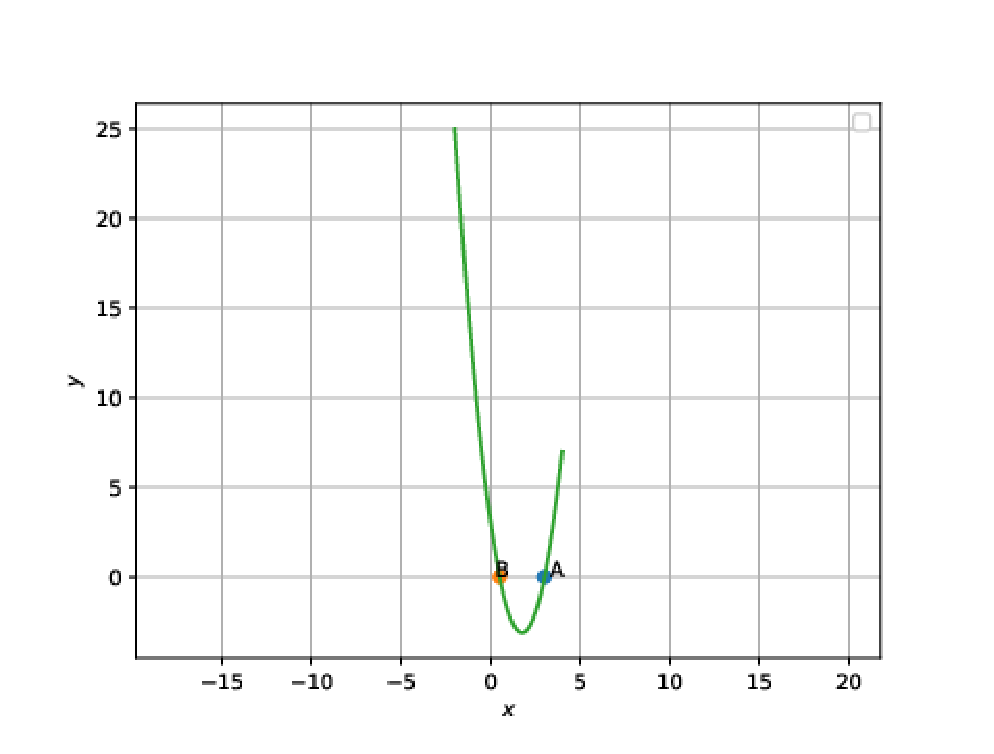
\includegraphics[width= \columnwidth]{./solutions/7/figs/conics/parabola1.eps}
\caption{Roots of $2x^2 - 7x + 3 = 0$}
\label{fig:5.2.7_par1}
\end{figure}
The python code can be downloaded from
\begin{lstlisting}
solutions/7/codes/conics/parabola1.py
\end{lstlisting}

\item 
$2x^2 + x -4 = 0$ can be expressed as 
\begin{align}
\label{eq:5.2.7_vec_conic_b}
\vec{x}^T \myvec{2 & 0\\0 & 0}\vec{x}+ \myvec{1 & 0}\vec{x} -4=0
\end{align}

From the \ref{fig:5.2.7_fig2}, the roots are 1.186 and 1.686.
\begin{figure}[!ht]
\centering
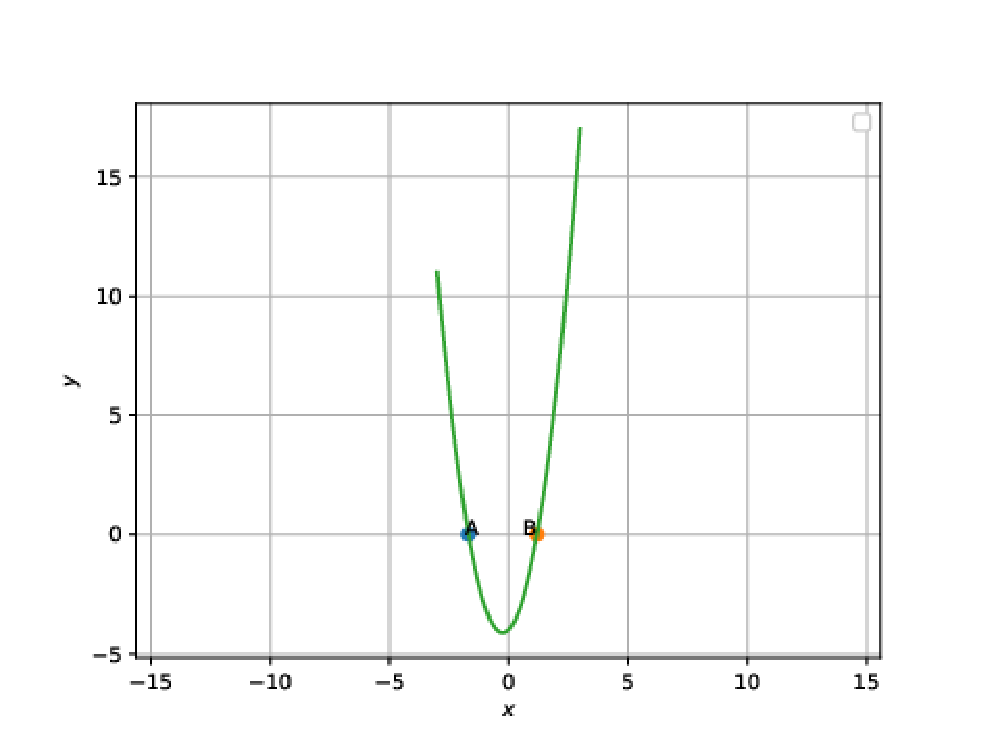
\includegraphics[width= \columnwidth]{./solutions/7/figs/conics/parabola2.eps}
\caption{Roots of $2x^2 + x -4 = 0$ }
\label{fig:5.2.7_fig2}
\end{figure}
The python code can be downloaded from
\begin{lstlisting}
solutions/7/codes/conics/parabola2.py
\end{lstlisting}

\item 
$4x^2 + 4\sqrt{3}x + 3 = 0$ can be expressed as 
\begin{align}
\label{eq:5.2.7_vec_conic_c}
\vec{x}^T \myvec{4 & 0\\0 & 0}\vec{x}+ \myvec{4\sqrt{3} & 0}\vec{x}+3=0
\end{align}
From the graph in \ref{fig:5.2.7_fig3}, the roots are real and equal. The root is $\frac{-\sqrt{3}}{2}$.
\begin{figure}[!ht]
\centering
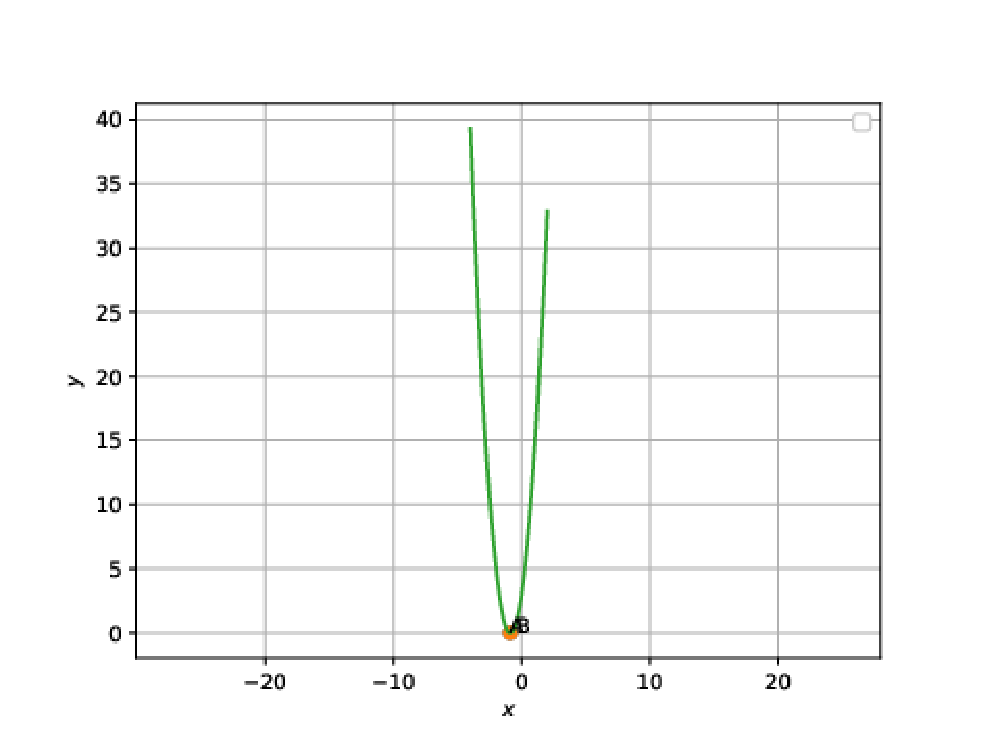
\includegraphics[width= \columnwidth]{./solutions/7/figs/conics/parabola3.eps}
\caption{Roots of $4x^2 + 4\sqrt{3}x + 3 = 0$}
\label{fig:5.2.7_fig3}
\end{figure}
The python code can be downloaded from
\begin{lstlisting}
solutions/7/codes/conics/parabola3.py
\end{lstlisting}

\item 
$2x^2 +x + 4 = 0$ can be expressed as 
\begin{align}
\label{eq:5.2.7_vec_conic_d}
\vec{x}^T \myvec{2 & 0\\0 & 0}\vec{x}+ \myvec{1 & 0}\vec{x}+4=0
\end{align}
From the graph \ref{fig:5.2.7_fig4}, the quadratic equation doesn't intersect x-axis. Thus it doesn't have real roots. It has ccomplex and conjugate roots.
\begin{figure}[!ht]
\centering
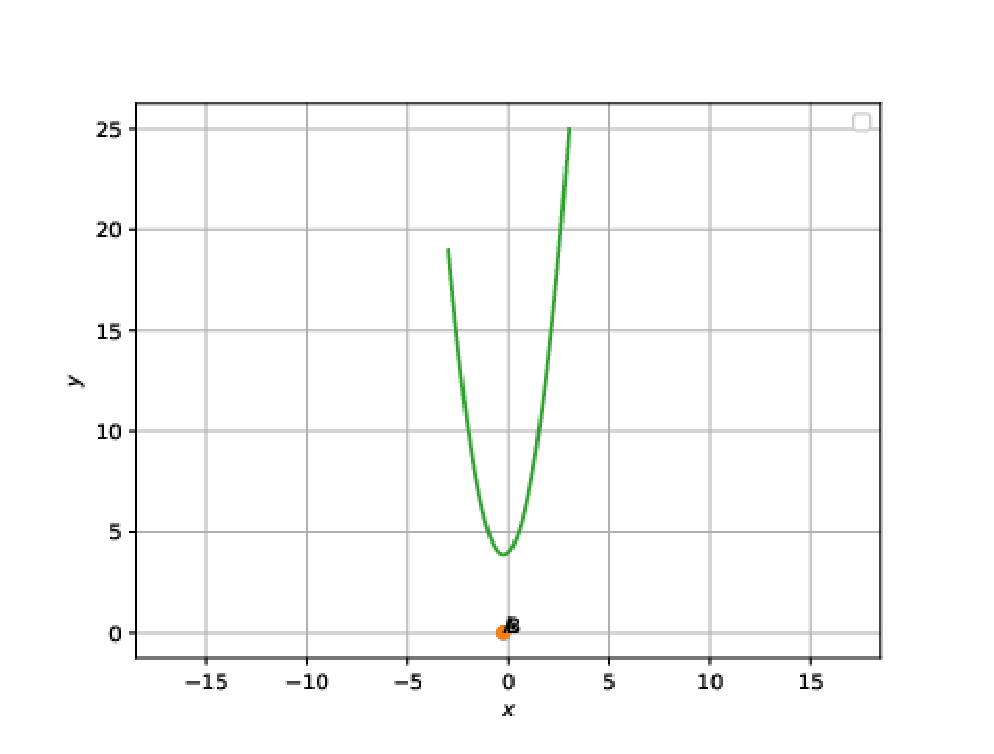
\includegraphics[width= \columnwidth]{./solutions/7/figs/conics/parabola4.eps}
\caption{Roots of $2x^2 +x + 4 = 0$ }
\label{fig:5.2.7_fig4}
\end{figure}
The python code can be downloaded from
\begin{lstlisting}
solutions/7/codes/conics/parabola4.py
\end{lstlisting}

\end{enumerate}
